\documentclass[a4paper,12pt]{report}

% --- PREAMBOLO ---
\usepackage[utf8]{inputenc}
\usepackage{lmodern}
\usepackage[T1]{fontenc}
\usepackage[italian]{babel}
\usepackage{graphicx}
\usepackage{geometry}
\geometry{a4paper, top=3cm, bottom=3cm, left=3.5cm, right=2.5cm}
\usepackage{amsmath}
\usepackage{amssymb}
\usepackage{cite}
\usepackage{microtype}
\usepackage{titlesec}
\usepackage{url}
\usepackage{hyperref}
\usepackage{tikz}
\usetikzlibrary{shapes,arrows,fit,positioning}
\usepackage{setspace}
\onehalfspacing

% Percorso immagini
\graphicspath{{./img/}}

\usepackage{titlesec}

% 1. Definisci lo stile (opzionale, ma serve per mantenere l'aspetto standard "Capitolo X")
\titleformat{\chapter}[display]
  {\normalfont\huge\bfseries\centering}   % Stile del testo (grassetto, enorme)
  {\chaptertitlename\ \thechapter} % Scrive "Capitolo 1"
  {20pt}                        % Spazio tra "Capitolo 1" e il titolo "Introduzione"
  {\Huge}                       % Dimensione del titolo del capitolo

% 2. Definisci gli spazi
\titlespacing*{\chapter}
  {0pt}   % Spazio a sinistra (rientro)
  {-30pt} % Spazio SOPRA il titolo (usa valori negativi per spostarlo in alto)
  {20pt}  % Spazio SOTTO il titolo (prima che inizi il testo)


\begin{document}

% --- A. FRONTESPIZIO (Dati dal PDF) ---
\begin{titlepage}
    \centering
    \vspace*{1cm}
    
    {\LARGE \textbf{UNIVERSITÀ DEGLI STUDI DI ROMA\\TOR VERGATA}} \\
    \vspace{0.5cm}
    {\Large Macroarea di Ingegneria} \\
    \vspace{0.2cm}
    {\large Corso di Studio in Ingegneria dell'Automazione} \\
    \vspace{2cm}

    {\Large Tesi di Laurea in \\ Analisi e Sintesi di Sistemi Non Lineari} \\
    \vspace{2cm}

    {\Huge \textbf{}} \\
    
    \vspace{3cm}

    \begin{minipage}[t]{0.45\textwidth}
        \raggedright \large
        \textbf{Relatore:}\\
        Chiar.mo Prof.\\ Daniele Carnevale\\
        \vspace{0.5cm}
        \textbf{Correlatore:}\\
        
    \end{minipage}
    \hfill
    \begin{minipage}[t]{0.45\textwidth}
        \raggedleft \large
        \textbf{Laureanda:}\\
        
    \end{minipage}

    \vfill
    {\large Anno Accademico 2025/2026}
\end{titlepage}

% --- B. INDICE ---
\pagenumbering{roman}
\tableofcontents
\listoffigures
\newpage

% --- C. CORPO DELLA TESI (Struttura PDF) ---
\pagenumbering{arabic}

% CAPITOLO 1
\chapter{Introduzione}
\label{ch:introduzione}
% \input{capitoli/1_introduzione} % Crea questo file se hai il testo

% CAPITOLO 2
\chapter{Stato dell'Arte}
\label{ch:stato_arte}
% !TEX root = ../main.tex

\section{Panoramica sugli UAV VTOL}

\subsection{Configurazioni principali}
La categoria degli UAV a decollo e atterraggio verticale (VTOL) è vasta e si articola principalmente in tre configurazioni strutturali, ognuna con specifici vantaggi e limitazioni operative:
\begin{itemize}
    \item \textbf{Multirotori:} Questa classe è caratterizzata da una notevole semplicità meccanica e dalla capacità di mantenere un \textit{hovering} estremamente stabile. Tuttavia, soffrono di una bassa efficienza energetica nel volo traslato, cosa che ne limita notevolmente l'autonomia e il raggio d'azione.
    \item \textbf{Ala fissa:} I velivoli ad ala fissa convenzionali offrono un'elevata efficienza aerodinamica, permettendo lunghe percorrenze e velocità di crociera elevate. Il loro svantaggio principale risiede nella necessità di infrastrutture dedicate o spazi ampi per le manovre di decollo e atterraggio, precludendone l'uso in ambienti confinati.
    \item \textbf{Ibridi:} Questa categoria nasce per combinare la versatilità operativa dei multirotori con l'efficienza dei velivoli ad ala fissa. Include architetture complesse come i \textit{tilting-rotor}, \textit{tilting-wing} e \textit{tailsitter}, capaci di transire tra le modalità di volo verticale e orizzontale.
\end{itemize}

\subsection{Sfide di modellazione e controllo}
Lo sviluppo di velivoli VTOL ibridi presenta sfide ingegneristiche significative, concentrate prevalentemente nella gestione della fase di transizione tra il volo verticale e quello orizzontale. In questo regime, il velivolo è soggetto a forti non linearità aerodinamiche causate dall'interazione complessa tra i flussi dei rotori, le superfici alari e la fusoliera.
Una modellazione efficace deve catturare accuratamente fenomeni quali gli effetti giroscopici, le variazioni repentine di portanza e resistenza, e il forte accoppiamento tra i gradi di libertà longitudinale e laterale. 
Di conseguenza, i sistemi di controllo devono essere progettati per garantire robustezza e prestazioni elevate durante tutte le fasi di volo, adattandosi a condizioni operative che variano drasticamente tra l'hovering statico e la crociera aerodinamica.

\clearpage
\section{UAV VTOL con ali indipendentemente inclinabili}
Un contributo significativo nello sviluppo di configurazioni ibride innovative è stato presentato in \cite{nam2020}, dove viene proposto un UAV VTOL caratterizzato da ali inclinabili in modo indipendente. L'obiettivo primario di tale design è superare i limiti di manovrabilità dei tricotteri classici e mitigare la coppia di reazione tipicamente gestita dal rotore di coda.
\\Dal punto di vista della modellazione, è stato derivato un modello dinamico a sei gradi di libertà (6-DOF) basato sulla formulazione di Newton-Eulero. Il modello evidenzia come il controllo differenziale dell'angolo di inclinazione (\textit{tilt}) delle due ali generi una differenza di portanza in grado di indurre momenti di rollio, sfruttando le forze propulsive in combinazione con quelle aerodinamiche.
\\La strategia di controllo implementata si basa su regolatori PID e PI integrati nel firmware Ardupilot, strutturati in base alla fase di volo:
\begin{itemize}
    \item \textbf{Modalità Verticale:} Vengono impiegati PID classici per la stabilizzazione di rollio, beccheggio e imbardata, allocando i comandi su tre motori brushless e tre servocomandi.
    \item \textbf{Modalità Orizzontale:} Il controllo del rollio è affidato alla variazione differenziale del tilt alare, il beccheggio è gestito tramite il rotore di coda (spinta e inclinazione vettoriale), mentre l'imbardata è stabilizzata da un controllore PI che minimizza lo scivolamento laterale (\textit{sideslip}).
\end{itemize}
La transizione è governata da una logica a stati finiti che coordina l'inclinazione progressiva delle ali, garantendo una traiettoria fluida durante il cambio di configurazione.

\clearpage
\section{Modellazione e controllo Backstepping per Quadricotteri}
In \cite{mian2008}, viene affrontato il problema del controllo non lineare per quadricotteri attraverso la derivazione di un modello completo a 6-DOF che include effetti giroscopici e dinamica degli attuatori. L'analisi sottolinea la natura sottattuata e fortemente accoppiata del sistema.
La strategia di controllo proposta adotta un approccio sequenziale ibrido:
\begin{itemize}
    \item Per il \textbf{sottosistema traslazionale} (posizione e altitudine), viene utilizzata una tecnica di linearizzazione con retroazione accoppiata a un regolatore PD.
    \item Per il \textbf{sottosistema rotazionale} (assetto), viene implementato un controllore non lineare basato sulla tecnica \textit{Backstepping} integrata con un'azione integrale (PID).
\end{itemize}
L'uso del Backstepping garantisce la stabilità asintotica globale, dimostrata tramite funzioni di Lyapunov, e offre una robustezza superiore rispetto ai PID tradizionali, specialmente nella reiezione dei disturbi esterni e nella riduzione dell'errore di inseguimento a regime.

\clearpage
\section{Controllo Sliding Mode "Smoothed" e Non-Overshooting}
Un'evoluzione recente per affrontare simultaneamente il problema del \textit{chattering} e quello delle sovraelongazioni (\textit{overshoot}) nella risposta dinamica degli UAV è presentata in \cite{Wang2024}.
Gli autori propongono una strategia di controllo robusta denominata \textit{Smoothed Non-overshooting Sliding Mode Control}, progettata per garantire la stabilità esponenziale globale anche in presenza di disturbi stocastici limitati.

A differenza degli approcci classici, che utilizzano una funzione di saturazione lineare a tratti ($\text{sat}(s)$) per mitigare il chattering, questo metodo impiega una funzione basata sulla tangente iperbolica ($\tanh(\cdot)$).
La legge di controllo assume la forma generale:
\begin{equation}
    u(t) = -k \cdot \tanh(\rho \cdot s(t))
\end{equation}
dove $\rho$ è un parametro di sintonizzazione che determina la pendenza della funzione.
I vantaggi principali di questa formulazione includono:
\begin{itemize}
    \item \textbf{Continuità e Derivabilità:} L'uso della $\tanh(\cdot)$ rende il segnale di controllo una funzione liscia (\textit{smooth}) e ovunque differenziabile. Questo elimina le discontinuità nella derivata che si verificano ai bordi dello strato limite nella funzione $\text{sat}(\cdot)$, riducendo lo stress meccanico sugli attuatori e migliorando la precisione di tracking.
    \item \textbf{Approssimazione Universale:} Viene dimostrato che per valori sufficientemente elevati di $\rho$, la funzione $\tanh(\rho \cdot s)$ approssima la funzione $\text{sign}(s)$ ideale, permettendo di recuperare le proprietà di robustezza dello SMC puro pur mantenendo un comportamento continuo.
    \item \textbf{Assenza di Overshoot:} La struttura del controllore è progettata con due sottosistemi sequenziali (raggiungibilità e stabilità) che garantiscono che la variabile di errore converga a zero senza mai superare il target, una caratteristica critica per la sicurezza nelle manovre UAV in ambienti ostili.
\end{itemize}

\clearpage
\section{Modellazione e Controllo Robusto per UAV Coaxial Tilting-Rotor}
Un'evoluzione significativa nel panorama dei velivoli a decollo verticale è rappresentata dalla configurazione \textit{Coaxial Tilting-Rotor} (CTRUAV), analizzata in \cite{cheng2022}. Questa architettura si distingue per la presenza di due coppie di rotori coassiali inclinabili posizionati nella parte anteriore del velivolo e un rotore fisso in coda. Rispetto ai tricotteri convenzionali, l'impiego di rotori coassiali permette di generare una spinta maggiore senza aumentare le dimensioni del telaio, migliorando la manovrabilità e annullando naturalmente il momento giroscopico grazie alla configurazione controrotante.
\begin{figure}[h]
    \centering
    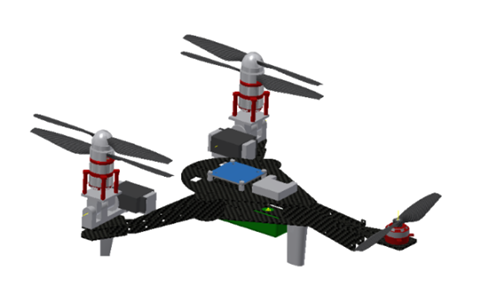
\includegraphics[width=0.5\textwidth]{coaxial}
    \caption{Coaxial tilting rotor UAV.}
    \label{fig:coaxial}
\end{figure}
Il modello dinamico a sei gradi di libertà è derivato utilizzando le formule di Newton-Eulero. Per governare questo sistema in presenza di disturbi esterni, è stata proposta una strategia di controllo gerarchica:
\begin{itemize}
    \item \textbf{Loop Esterno (Posizione):} Per il tracking della traiettoria desiderata, viene impiegato un controllore basato sulla tecnica del \textit{Backstepping}, che stabilizza asintoticamente l'errore di posizione.
    \item \textbf{Loop Interno (Assetto):} La stabilizzazione è affidata a un controllore \textit{Robust Adaptive Backstepping Sliding Mode} (ABSMC). L'integrazione di una legge adattiva permette di stimare online il limite superiore dei disturbi esterni. Tale stima modula il guadagno della legge di controllo, minimizzando il fenomeno del \textit{chattering} tramite l'uso di funzioni di saturazione.
\end{itemize}
Le simulazioni dimostrano che l'approccio proposto garantisce una robustezza superiore rispetto ai controllori backstepping tradizionali.

\clearpage
\section{Strategie di Volo e Controllo per Tricotteri Tilting-Rotor}
In \cite{chen2017}, l'attenzione si sposta sulla realizzazione pratica di un volo autonomo "full-mode" per un UAV tilting-rotor in configurazione tricottero compatta. L'obiettivo è superare le limitazioni di costo associate all'ottenimento di modelli dinamici precisi, proponendo una strategia robusta che non dipenda da dati aerodinamici ad alta fedeltà.
\\La gestione del volo è affidata a una strategia basata su una macchina a stati finiti che coordina le diverse fasi: \textit{Rotor mode} (decollo verticale), \textit{Conversion} (transizione accelerata), \textit{Fixed-wing mode} (crociera) e \textit{Reconversion} (ritorno all'hovering).
Un elemento centrale è il sistema di \textbf{Motor Mixing Algorithm}; poiché il sistema è sovra-attuato e non affine durante la transizione, il mixer distribuisce i pesi di controllo tra modalità rotore e ala fissa in base all'efficienza degli attuatori e all'angolo di tilting corrente. Una peculiarità è il controllo dell'imbardata in hovering tramite tilt differenziale dei rotori anteriori, che viene disattivato progressivamente durante la transizione.
I test di volo reali hanno validato la capacità del velivolo di eseguire l'intero inviluppo di volo mantenendo la stabilità \cite{chen2017}.
\begin{figure}[h]
        \centering
        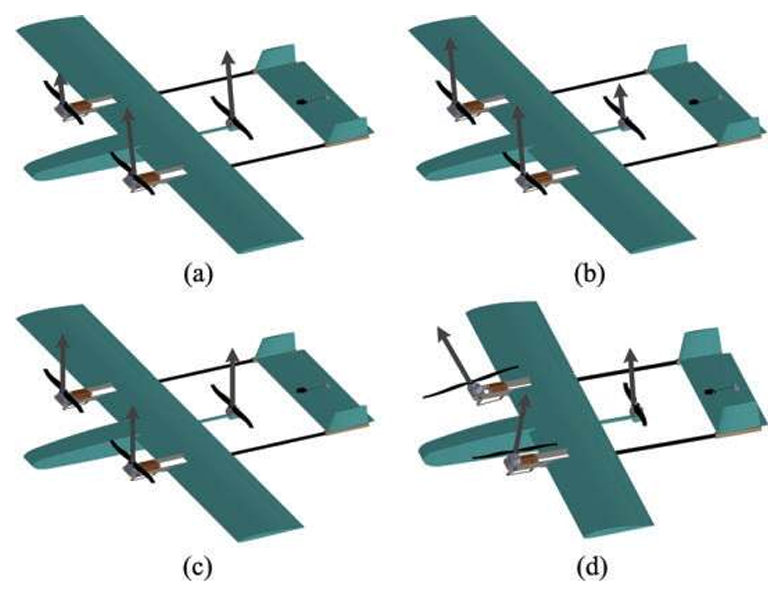
\includegraphics[width=0.5\textwidth]{paper5.png}
        \caption{Control logic in rotor mode. (a) roll, (b) pitch, (c) thrust, and (d) yaw.}
        \label{fig:paper5}
\end{figure}

\clearpage
\section{Controllo Sliding Mode a Tempo Fisso}
La problematica della convergenza rapida e garantita è affrontata in \cite{yu2022}, dove viene proposto uno schema per la stabilizzazione dell'assetto di un \textit{Tilting Trirotor UAV} basato sulla stabilità a tempo fisso (\textit{Fixed-Time Stability}). A differenza della stabilità asintotica o a tempo finito, questo approccio garantisce che il sistema raggiunga l'equilibrio entro un tempo limitato, noto a priori e indipendente dallo stato iniziale.
\\Il contributo teorico principale è la formulazione di un \textit{Novel Fixed-Time Stable System} che dimostra un tasso di convergenza superiore rispetto ai metodi esistenti. Basandosi su questo, è stato sviluppato uno schema \textit{Nonsingular Fixed-Time Sliding Mode Control} (NFTSMC) che include:
\begin{itemize}
    \item \textbf{Superficie di Scorrimento Non Singolare:} Progettata per evitare le singolarità matematiche tipiche dei controllori terminali e garantire la convergenza.
    \item \textbf{Tecnica Adattiva per i Disturbi:} Una legge di aggiornamento stima i disturbi in tempo reale, assicurando robustezza.
\end{itemize}
La validazione sperimentale su prototipo reale ha confermato una convergenza degli errori di assetto in meno di 0,3 secondi e una notevole reiezione dei disturbi \cite{yu2022}.

\clearpage
\section{Controllo tramite Spinta Differenziale}
Un aspetto tecnologico cruciale esplorato in \cite{riboldi2023} è la completa sostituzione delle superfici di controllo aerodinamiche convenzionali (alettoni, elevatori, timoni) con una logica di controllo basata esclusivamente sulla modulazione della spinta (\textit{Differential Thrust}).
Questa architettura richiede l'impiego di propulsori in grado di fornire spinta reversibile (positiva e negativa), permettendo la generazione di momenti di controllo anche a velocità nulla, una capacità preclusa ai sistemi aerodinamici tradizionali.
\\La strategia di (\textit{mixing}) mappa i comandi di assetto desiderati (Rollio, Beccheggio, Imbardata) direttamente sulle coppie di motori, secondo lo schema seguente (riferito a una configurazione a quattro propulsori disposti a "X"):
\begin{itemize}
    \item \textbf{Controllo di Beccheggio (Pitch):} Sostituisce la funzione dell'elevatore. Viene generato creando una spinta differenziale tra i rotori superiori e quelli inferiori. Ad esempio, per cabrare, i propulsori inferiori generano spinta positiva mentre quelli superiori generano spinta negativa, creando una coppia pura sull'asse trasversale.
    \item \textbf{Controllo di Imbardata (Yaw):} Sostituisce il timone verticale. Si ottiene differenziando la spinta tra i motori di destra e quelli di sinistra. Una rotazione verso destra è indotta da una spinta positiva sui motori di sinistra e negativa su quelli di destra.
    \item \textbf{Controllo di Rollio (Roll):} Sostituisce gli alettoni. A differenza dei velivoli ad ala fissa dove il rollio è generato alle estremità alari, qui viene prodotto tramite una configurazione incrociata. Ad esempio, una spinta positiva del motore in basso a destra combinata con il motore in alto a sinistra, opposta alla coppia degli altri due, genera il momento torcente longitudinale necessario \cite{riboldi2023}.
\end{itemize}
Questa metodologia offre il vantaggio di eliminare attuatori meccanici complessi (servocomandi) e parti mobili, riducendo il peso strutturale e la manutenzione. Tuttavia, introduce una maggiore complessità nel software di controllo, poiché i gradi di libertà risultano fortemente accoppiati: una singola manovra richiede spesso la modulazione simultanea di tutti i propulsori per evitare effetti secondari indesiderati sugli altri assi. 

% CAPITOLO 3
\chapter{Modello Matematico}
\label{ch:modello}
% !TEX root = ../main.tex

\section{Sistemi di Riferimento}
Per descrivere la dinamica del tricottero VTOL, si adottano due sistemi di riferimento principali, entrambi destrorsi:
\begin{itemize}
    \item \textbf{Sistema Inerziale (Earth Frame) $\mathcal{F}_g$}: Fisso rispetto al terreno, definito dalla terna $(O_g, X_g, Y_g, Z_g)$. La posizione del velivolo è indicata dal vettore $P_g = [x_g, y_g, z_g]^T$ e l'orientamento dagli angoli di Eulero $\Theta_g = [\phi, \theta, \psi]^T$ (Roll, Pitch, Yaw).
    \item \textbf{Sistema Solidale (Body Frame) $\mathcal{F}_b$}: Con origine nel centro di massa (CoM) del velivolo e assi $(X_b, Y_b, Z_b)$ solidali alla struttura. Le velocità lineari e angolari sono definite rispettivamente come $V_b = [u, v, w]^T$ e $\Omega_b = [p, q, r]^T$.
\end{itemize}
\begin{figure}[h]
    \centering
    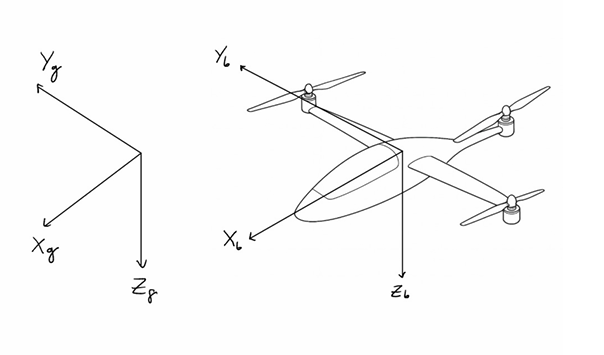
\includegraphics[width=0.7\textwidth]{sist_rif.png}
    \caption{Sistemi di riferimento.}
    \label{fig:sist_rif}
\end{figure}
La trasformazione delle velocità lineari dal sistema solidale al corpo a quello inerziale avviene tramite la matrice di rotazione $R_{b \to g}$ (convenzione ZYX):
\begin{equation}
    \dot{P}_g = R_{b \to g}(\Theta_g) V_b
\end{equation}
Analogamente, la relazione cinematica tra le velocità angolari del corpo e le derivate degli angoli di Eulero è data dalla matrice di trasformazione $J_{b \to g}$:
\begin{equation}
    \dot{\Theta}_g = J_{b \to g}(\Theta_g) \Omega_b
\end{equation}

\section{Equazioni della Dinamica}
Il modello dinamico è derivato utilizzando la formulazione di Newton-Eulero per un corpo rigido a 6 gradi di libertà. Le equazioni vettoriali che descrivono il moto traslazionale e rotazionale sono:

\begin{equation}
    \begin{cases}
        m \dot{V}_b + \Omega_b \times (m V_b) = F_{\mathrm{tot}} \\
        I_b \dot{\Omega}_b + \Omega_b \times (I_b \Omega_b) = M_{\mathrm{tot}}
    \end{cases}
    \label{eq:newton_euler}
\end{equation}
\begin{itemize}
    \item $m$ è la massa totale del velivolo,
    \item $I_b$ è il tensore d'inerzia (assunto diagonale per simmetria strutturale), 
    \item $F_{\mathrm{tot}}$ e $M_{\mathrm{tot}}$ sono rispettivamente la somma delle forze e dei momenti esterni agenti sul corpo, espressi nel \textit{body frame}.

\end{itemize} 

\section{Analisi delle Forze}
Le forze agenti sul tricottero sono la risultante della spinta dei motori ($F_{\mathrm{th}}$), della forza di gravità ($F_g$) e delle forze aerodinamiche ($F_{\mathrm{aero}}$):
\begin{equation}
    F_{\mathrm{tot}} = F_{\mathrm{th}} + F_g + F_{\mathrm{aero}}
\end{equation}

\subsection{Thrust}
Il velivolo è dotato di tre rotori: due anteriori (1 e 2) e uno posteriore (3).
\begin{itemize}
    \item I rotori anteriori possono inclinarsi (\textit{tilt}) attorno all'asse $Y_b$ di un angolo $\theta_1$ e $\theta_2$.
    \item Il rotore di coda possiede due gradi di libertà, potendo ruotare attorno a $Y_b$ ($\theta_3$) e $Z_b$ ($\theta_4$).
\end{itemize}
Ogni rotore genera una spinta $f_i = k \omega_i^2$ lungo il proprio asse di rotazione. Il vettore forza totale, espresso nel body frame, si ottiene sommando i contributi dei tre rotori ruotati dalle rispettive matrici di tilt:
\begin{figure}[h]
    \centering
    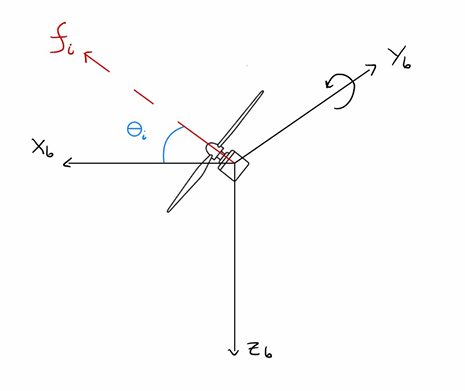
\includegraphics[width=0.6\textwidth]{rotori_1_2.png}
    \caption{Direzione (in rosso) del thrust per i rotori 1 e 2 nel piano $(X_{b}, Z_{b})$.}
    \label{fig:rotori_1_2}
\end{figure}

\begin{figure}[H]
    \centering
    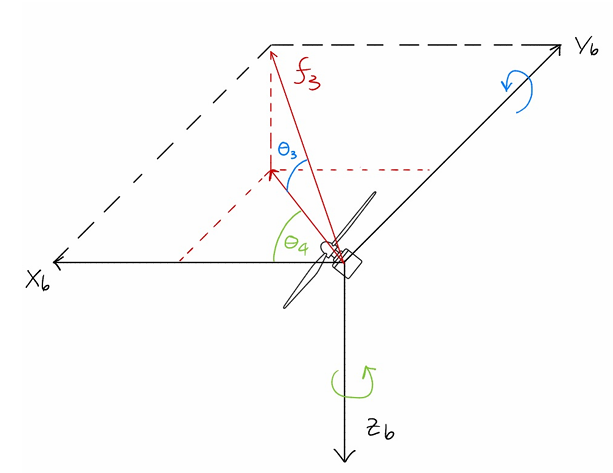
\includegraphics[width=0.7\textwidth]{rotore_3.png}
    \caption{Direzione (in rosso) del thrust per il rotore 3 nei piani $(X_{b}, Z_{b})$ e $(X_{b}, Y_{b})$.}
    \label{fig:rotore_3}
\end{figure}

\begin{equation}
    F_{\mathrm{th}} = \sum_{i=1}^{3} R_{\mathrm{tilt}, i} \cdot \begin{bmatrix} 0 \\ 0 \\ -f_i \end{bmatrix}
\end{equation}
Espandendo i termini, la forza risultante assume la forma:
\begin{equation}
    F_{\mathrm{th}} = 
    \begin{bmatrix}
    c_{\theta_1} f_1 + c_{\theta_2} f_2 + c_{\theta_3} c_{\theta_4} f_3 \\
    c_{\theta_3} s_{\theta_4} f_3 \\
    -s_{\theta_1} f_1 - s_{\theta_2} f_2 - s_{\theta_3} f_3
    \end{bmatrix}
\end{equation}
dove si è usata la notazione abbreviata $c_\alpha = \cos\alpha$ e $s_\alpha = \sin\alpha$.

\subsection{Gravità e Aerodinamica}
La forza peso, costante nel sistema inerziale, viene ruotata nel sistema solidale al corpo:
\begin{equation}
    F_g = R_{b \to g}^T \begin{bmatrix} 0 \\ 0 \\ mg \end{bmatrix} = mg \begin{bmatrix} -\sin\theta \\ \cos\theta \sin\phi \\ \cos\theta \cos\phi \end{bmatrix}
\end{equation}
Le forze aerodinamiche (Portanza $L$ e Resistenza $D$) agenti sulle superfici alari sono modellate in funzione della pressione dinamica e dei coefficienti aerodinamici $C_L$ e $C_D$:
\begin{equation}
    F_{\mathrm{aero}} \approx 
    \begin{bmatrix}
        -\frac{1}{2}\rho S C_D v_x |v_x| \\
        0 \\
        -\frac{1}{2}\rho S C_L v_x^2 - \frac{1}{2}\rho S C_{D_z} v_z |v_z|
    \end{bmatrix}
\end{equation}
Si assume per semplicità che il moto laterale non generi forze aerodinamiche significative sulle ali principali.

\section{Analisi dei Momenti}
Il momento totale agente sul baricentro è la somma di diverse componenti:
\begin{equation}
    M_{\mathrm{tot}} = M_{\mathrm{th}} + M_{\mathrm{drag}} + M_{\mathrm{aero}} + M_{\mathrm{gyro}} + M_{\mathrm{fin}}
\end{equation}

\subsection{Momenti generati dai Rotori}
Il contributo principale è dato dal momento generato dalla spinta dei rotori, calcolato come il prodotto vettoriale tra i bracci di leva $r_i$ (distanza del rotore dal CoM) e le forze di spinta $F_{\mathrm{th},i}$:
\begin{equation}
    M_{\mathrm{th}} = \sum_{i=1}^{3} (r_i \times F_{\mathrm{th},i})
\end{equation}
Inoltre, la rotazione delle eliche genera un momento torcente ($M_{\mathrm{drag}}$) opposto al verso di rotazione, proporzionale al quadrato della velocità angolare ($\tau_i = b \omega_i^2$). Poiché i rotori sono inclinabili, anche questo momento viene proiettato sugli assi del body frame in funzione degli angoli di tilt.

\subsection{Effetti Aerodinamici e Giroscopici}
\begin{itemize}
    \item \textbf{Momento Aerodinamico ($M_{\mathrm{aero}}$):} È generato dalle forze di portanza e resistenza applicate nel centro di pressione delle ali, che non coincide con il centro di massa. Questo crea coppie di beccheggio e rollio in funzione della velocità di avanzamento.
    \item \textbf{Momento Giroscopico ($M_{\mathrm{gyro}}$):} Dovuto alla precessione giroscopica dei rotori ad alta velocità quando il velivolo (o i rotori stessi tramite il meccanismo di tilt) ruota. È dato da:
    \begin{equation}
        M_{\mathrm{gyro}} = \sum_{i=1}^{3} I_{\mathrm{rot}} (\Omega_b \times \hat{e}_{\mathrm{rot},i}) \omega_i
    \end{equation}
    \item \textbf{Momento della Pinna ($M_{\mathrm{fin}}$):} La superficie verticale di coda genera un momento stabilizzante di imbardata e un momento di rollio indotto, modellati in funzione delle velocità angolari $p, r$ e della velocità laterale.
\end{itemize}
L'insieme di queste equazioni definisce il modello matematico completo utilizzato per la sintesi del controllo nel Capitolo \ref{ch:controllo}. % Qui andrebbero le equazioni di moto (Thrust, Gravità)

% CAPITOLO 4
\chapter{Dimostrazione SMC}
\label{ch:dimostrazione}
% --- Sezione Controllo Verticale ---
\section{\hbox{Analisi di Lyapunov per il controllo verticale}}
Di seguito è analizzata la stabilità secondo Lyapunov del sistema d'errore attraverso l'applicazione della legge di controllo \textit{Sliding Mode} sviluppata per il volo verticale. Si considera, a titolo esemplificativo, il caso lungo l'asse $z$.\\
Si adotta un sistema di riferimento \textbf{NED (North-East-Down)}, in cui l'asse $z$ è orientato verso il centro della Terra; pertanto, valori di $z$ positivi indicano una quota crescente verso il basso.

\subsection{Modellazione della Dinamica}
La dinamica del sistema viene analizzata nel frame inerziale, poiché il loop di controllo esterno si basa sull'errore di posizione, che perde di significato nel body frame.\\
Il secondo principio della dinamica, proiettato sull'asse $z$ del sistema inerziale, definisce l'evoluzione del velivolo come:
\begin{equation}
    m\ddot{z} = mg + \cos(\phi)\cos(\theta) F_{\mathrm{aero},z} - \cos(\phi)\cos(\theta) F_{\mathrm{thrust},z} + d(t)
    \label{eq:dynamics_z_final}
\end{equation}
dove:
\begin{itemize}
    \item $m$ è la massa totale del velivolo;
    \item $g$ è l'accelerazione di gravità (positiva nel riferimento NED);
    \item $F_{\mathrm{thrust},z}$ è la componente verticale della spinta, ovvero l'ingresso di controllo;
    \item $F_{\mathrm{aero},z} = -\frac{1}{2}\rho S C_d \operatorname{sgn}(\dot{z})\dot{z}^2$ rappresenta la resistenza aerodinamica lungo l'asse verticale;
    \item $d(t)$ rappresenta le incertezze di modello e i disturbi esterni non modellati.
\end{itemize}
Normalizzando rispetto alla massa, si ottiene la forma affine al controllo:
\begin{equation}
    \ddot{z} = g + \cos(\phi)\cos(\theta) \left(\frac{F_{\mathrm{aero},z}}{m} - \frac{u}{m} \right) + \Delta(t)
\end{equation}
In questa formulazione, $\Delta(t) = d(t)/m$ è definita come \textbf{incertezza matched}, in quanto agisce direttamente sullo stesso canale dell'ingresso di controllo $u = F_{\mathrm{thrust},z}$. Si assume che tale disturbo sia limitato superiormente da una costante nota: \hbox{$|\Delta(t)| \le \Delta_{\max}$}, $\forall t \ge 0$.

\subsection{Definizione della \textit{sliding surface}}
Sia $z_{\mathrm{des}}(t)$ la quota di riferimento desiderata e $e(t) = z_{\mathrm{des}}(t) - z(t)$ l'errore. Per un sistema del secondo ordine, si definisce una \textit{sliding surface} $\sigma(t)$ lineare del primo ordine:
\begin{equation}
    \sigma(t) = \dot{e}(t) + \lambda e(t)
\end{equation}
con $\lambda > 0$ costante di progetto. La condizione di regime $\sigma = 0$ definisce una dinamica vincolata (sliding mode) in cui l'errore decade esponenzialmente a zero. 

\subsection{Sintesi della Legge di Controllo}
Per ricavare la legge di controllo, si deriva rispetto al tempo la \textit{sliding surface} $\sigma(t)$, ottenendo $\dot{\sigma} = \ddot{z}_{\mathrm{des}} - \ddot{z} + \lambda \dot{e}$. Sostituendo l'espressione della dinamica del sistema proiettata lungo $z$, si ricava la dinamica dell'errore sulla superficie:
\begin{equation}
    \dot{\sigma} = \ddot{z}_{\mathrm{des}} - g - \cos(\phi)\cos(\theta)\frac{F_{\mathrm{aero},z}}{m} + \cos(\phi)\cos(\theta)\frac{u}{m} - \Delta(t) + \lambda \dot{e}
\end{equation}

L'obiettivo del controllo Sliding Mode è garantire che le traiettorie del sistema raggiungano la superficie $\sigma = 0$ in tempo finito. 
A tal fine, si adotta l'approccio basato sulla \textbf{reaching law}; si impone che la dinamica:
\begin{equation}
    \dot{\sigma} = -k \operatorname{sgn}(\sigma)
\end{equation}
con $k > 0$ parametro di progetto. Uguagliando la dinamica nominale alla legge di raggiungimento desiderata, si ottiene l'equazione algebrica da cui estrarre analiticamente l'ingresso di controllo $u$:
\begin{equation}
    \ddot{z}_{\mathrm{des}} - g - \cos(\phi)\cos(\theta)\frac{F_{\mathrm{aero},z}}{m} + \lambda \dot{e} + \cos(\phi)\cos(\theta)\frac{u}{m} = -k \operatorname{sgn}(\sigma)
\end{equation}

Isolando il termine dipendente dall'azione di controllo, si ottiene:
\begin{equation}
    \cos(\phi)\cos(\theta)\frac{u}{m} = -\ddot{z}_{\mathrm{des}} + g + \cos(\phi)\cos(\theta)\frac{F_{\mathrm{aero},z}}{m} - \lambda \dot{e} - k \operatorname{sgn}(\sigma)
\end{equation}

Si ricava la legge di controllo completa:
\begin{equation}
    u = \frac{m}{\cos(\phi)\cos(\theta)} \left( g - \ddot{z}_{\mathrm{des}} - \lambda \dot{e} \right) + F_{\mathrm{aero},z} - \frac{m}{\cos(\phi)\cos(\theta)} k \operatorname{sgn}(\sigma)
\end{equation}

Affinché l'inversione della dinamica sia matematicamente ben posta, è strettamente necessario introdurre l'assunzione che gli angoli di assetto soddisfino $\phi, \theta \in (-\pi/2, \pi/2)$. Fisicamente, questa condizione evita la singolarità cinematica, garantendo che il velivolo non si trovi in orientamento perfettamente verticale o capovolto, configurazione in cui la spinta non avrebbe alcuna componente utile lungo l'asse $z$ inerziale.

Una parte del controllo annulla la dinamica nota del sistema e assumiamo che i termini residui di queste cancellazioni vengano assorbiti dall'incertezza $\Delta(t)$; un'altra parte del controllo, 
ovvero il contributo discontinuo, impone la legge di raggiungimento.

Infine, applicando la legge di controllo $u$ così sintetizzata al sistema perturbato originale, la dinamica a ciclo chiuso proiettata sulla \textit{sliding surface} si riduce all'espressione:
\begin{equation}
    \dot{\sigma} = -k \operatorname{sgn}(\sigma) - \Delta(t)
\end{equation}
Questo è il punto di partenza per la dimostrazione formale della stabilità, in quanto il parametro $k$ dovrà essere dimensionato opportunamente per dominare il termine incerto $\Delta(t)$.


\subsection{Analisi di Stabilità e Tempo di Raggiungimento}
Per dimostrare la stabilità asintotica e la convergenza in tempo finito alla superficie, si introduce la funzione candidata di Lyapunov $V = \frac{1}{2}\sigma^2$. Dalla sua definizione si evince la relazione:
\begin{equation}
    \sqrt{2V} = |\sigma|
\end{equation}

Calcoliamo la derivata temporale lungo le traiettorie del sistema a ciclo chiuso. Sostituendo la dinamica di $\dot{\sigma}$:
\begin{align}
    \dot{V} &= \sigma \dot{\sigma} = \sigma \left( -k \operatorname{sgn}(\sigma) - \Delta(t) \right) \nonumber \\
            &= -k|\sigma| - \sigma \Delta(t)
\end{align}

Applicando la disuguaglianza triangolare e sapendo che il termine incerto è limitato superiormente ($|\Delta(t)| \le \Delta_{\max}$), si ottiene:
\begin{equation}
    \dot{V} \le -k|\sigma| + \Delta_{\max}|\sigma| = - (k - \Delta_{\max}) |\sigma|
\end{equation}

Definendo $\delta = k - \Delta_{\max}$, e ricordando che $|\sigma| = \sqrt{2V}$, possiamo riscrivere la disequazione differenziale direttamente in termini di $V$:
\begin{equation}
        \dot{V} = \sigma\dot{\sigma} \le -(k - \Delta_{\max})|\sigma| = -\delta \sqrt{2V}
\end{equation}
da cui ricaviamo che il guadagno deve essere $k = \Delta_{\max} + \delta$ per garantire la robustezza del controllo.
\begin{equation}
    \frac{dV}{dt} \le -\delta \sqrt{2V}
\end{equation}

Per dimostrare la convergenza in tempo finito, integriamo la disequazione per separazione di variabili. Separando i termini dipendenti da $V$ da quelli in $t$:
\begin{equation}
    \frac{dV}{\sqrt{V}} \le -\delta \sqrt{2} \, dt
\end{equation}

Integrando ambo i membri tra l'istante iniziale $t=0$ e un generico istante $t$:
\begin{equation}
    \int_{V(0)}^{V(t)} V^{-\frac{1}{2}} \, dV \le -\delta \sqrt{2} \int_{0}^{t} d\tau
\end{equation}

Risolvendo l'integrale si ottiene:
\begin{equation}
    2\sqrt{V(t)} - 2\sqrt{V(0)} \le -\sqrt{2} \, \delta \, t
\end{equation}

Dividendo ambo i membri per $\sqrt{2}$ e reintroducendo la relazione iniziale $\sqrt{2V} = |\sigma|$, l'espressione diventa:
\begin{equation}
    |\sigma(t)| - |\sigma(0)| \le - \delta \, t
\end{equation}

Da cui si definisce l'evoluzione dell'errore nel tempo:
\begin{equation}
    0 \le |\sigma(t)| \le |\sigma(0)| - \delta \, t
\end{equation}

Il tempo di raggiungimento $t_r$ coincide con il momento in cui le traiettorie intersecano per la prima volta la superficie, condizione per la quale si ha $|\sigma(t_r)| = 0$. Sostituendo questa condizione, si ricava il limite superiore per il tempo di convergenza:
\begin{equation}
    t_r \le \frac{|\sigma(0)|}{\delta}
\end{equation}

Questa dimostrazione prova che, scegliendo un guadagno $k$ sufficientemente grande per dominare le incertezze del modello, le traiettorie del sistema vengono forzate a raggiungere la \textit{sliding surface} in un tempo strettamente finito. Una volta sulla superficie ($\sigma=0$), il sistema esibisce la dinamica nominale asintoticamente stabile imposta da $\sigma = \dot{e} + \lambda e = 0$.

\subsection{Mitigazione del Chattering}

La natura discontinua della funzione $\operatorname{sgn}(\sigma)$ induce oscillazioni ad alta frequenza (chattering) che possono eccitare dinamiche non modellate e danneggiare gli attuatori. Per mitigare tale effetto, si introduce la regolarizzazione tramite un \textbf{boundary layer} di spessore $\Phi$, sostituendo la funzione segno con una funzione continua. In questo lavoro si utilizza la tangente iperbolica:
\begin{equation}
u = -k \tanh\left(\frac{\sigma}{\Phi}\right)
\end{equation}

Il parametro $\Phi>0$ definisce lo spessore dello strato limite attorno alla superficie di sliding. In particolare, si introducono le curve di livello
\begin{equation}
\begin{matrix}
L_{\Phi} = \{x : \sigma(x) = \Phi\} \\
L_{-\Phi} = \{x : \sigma(x) = -\Phi\}
\end{matrix}
\end{equation}

che delimitano il \textit{boundary layer}, definito come l'insieme
\begin{equation}
B = \{x \in \mathbb{R}^n : |\sigma(x)| \le \Phi \}.
\end{equation}

L'introduzione dello strato limite comporta la perdita della stabilità asintotica dell'origine. In presenza della regolarizzazione della legge di controllo, il sistema non converge esattamente alla superficie di sliding $\sigma=0$; tuttavia, le traiettorie raggiungono in \textit{tempo finito} un intorno della superficie di sliding e rimangono limitate al suo interno. Per questo motivo si parla di \textbf{stabilità pratica in tempo finito}. In particolare, come riportato in \cite{khalil2002nonlinear}, il sistema risulta \textit{uniformly ultimately bounded}, con un \textit{ultimate bound} la cui ampiezza dipende dal parametro $\Phi$ e dal guadagno del controllore.

Per dimostrare la convergenza verso lo strato limite, si consideri la funzione di Lyapunov candidata
\begin{equation}
V = \frac{1}{2}\sigma^2 .
\end{equation}

Si assuma che la dinamica della variabile di sliding possa essere scritta nella forma
\begin{equation}
\dot{\sigma} = -k \tanh\left(\frac{\sigma}{\Phi}\right) - \Delta(t)
\end{equation}

dove $\Delta(t)$ rappresenta disturbi e incertezze limitate tali che $|\Delta(t)| \le \Delta_{\max}$. La derivata della funzione di Lyapunov lungo le traiettorie del sistema risulta
\begin{equation}
\dot{V} = \sigma \dot{\sigma}
\end{equation}

da cui
\begin{equation}
\dot{V} = -k \sigma \tanh\left(\frac{\sigma}{\Phi}\right) - \sigma \Delta(t).
\end{equation}

Utilizzando il bound sul disturbo si ottiene
\begin{equation}
\dot{V} \le -k |\sigma| \tanh\left(\frac{|\sigma|}{\Phi}\right) + |\sigma| \Delta_{\max}
\end{equation}

ovvero
\begin{equation}
\dot{V} \le -|\sigma|\left(k \tanh\left(\frac{|\sigma|}{\Phi}\right) - \Delta_{\max}\right).
\end{equation}

Al di fuori dello strato limite vale la condizione $|\sigma|>\Phi$, da cui
\[
\frac{|\sigma|}{\Phi} > 1.
\]

Poiché la funzione $\tanh(x)$ è monotona crescente, segue che
\begin{equation}
\tanh\left(\frac{|\sigma|}{\Phi}\right) \ge \tanh(1).
\end{equation}
dove $\tanh(1)$ rappresenta il valore della funzione sul bordo del \textit{boundary layer}.

Pertanto si ottiene la stima
\begin{equation}
\dot{V} \le -|\sigma|\left(k\tanh(1)-\Delta_{\max}\right).
\end{equation}

Definendo $\eta = k \tanh(1) - \Delta_{\max}$, affinché $\dot{V}<0$ al di fuori dello strato limite è sufficiente imporre la seguente condizione sul guadagno del controllore:
\begin{equation}
k = \frac{\Delta_{\max} + \eta}{\tanh(1)}.
\end{equation}

Questa disuguaglianza garantisce che le traiettorie del sistema vengono attratte verso il \textit{boundary layer}.

Poiché $V=\frac{1}{2}\sigma^2$, si ha
\begin{equation}
|\sigma| = \sqrt{2V}.
\end{equation}

Sostituendo tale relazione nella stima precedente si ottiene
\begin{equation}
\dot{V} \le -\eta \sqrt{2V}.
\end{equation}

Questa disuguaglianza differenziale permette di stimare il tempo necessario affinché le traiettorie entrino nello strato limite. Integrando entrambi i membri si ottiene
\begin{equation}
\frac{dV}{\sqrt{V}} \le -\sqrt{2} \eta dt.
\end{equation}

Integrando tra $V(0)$ e $V(t)$ si ricava
\begin{equation}
2(\sqrt{V(t)}-\sqrt{V(0)}) \le -\sqrt{2}\eta t.
\end{equation}

Da cui si ottiene un limite superiore per il tempo necessario affinché la traiettoria raggiunga lo strato limite:
\begin{equation}
t_r \le \frac{|\sigma(0)|}{\eta}.
\end{equation}

Questo risultato dimostra che il sistema converge in \textit{tempo finito} verso il \textit{boundary layer}, confermando la \textbf{finite-time practical stability}.

Una volta entrate nello strato limite, l'argomento della tangente iperbolica è piccolo ($|\sigma|/\Phi \le 1$) e vale l'approssimazione lineare
\begin{equation}
\tanh(x) \approx x.
\end{equation}

La dinamica della variabile di sliding diventa quindi approssimativamente
\begin{equation}
\dot{\sigma} \approx -\frac{k}{\Phi}\sigma - \Delta(t),
\end{equation}

che rappresenta un sistema lineare stabile perturbato. In questa regione le traiettorie rimangono limitate all'interno dello strato limite, con un errore residuo la cui ampiezza dipende dal parametro $\Phi$ e dall'intensità dei disturbi. Riducendo opportunamente il valore di $\Phi$, tale errore può essere reso arbitrariamente piccolo.

In conclusione, emerge un fondamentale trade-off progettuale legato alla scelta dello spessore $\Phi$: un valore ridotto dello strato limite permette di minimizzare l'errore residuo a regime, avvicinando le prestazioni del sistema a quelle dello Sliding Mode ideale; tuttavia, ciò comporta una minore capacità di filtraggio delle oscillazioni ad alta frequenza. Al contrario, un valore di $\Phi$ più elevato garantisce una superiore mitigazione del chattering e una maggiore protezione degli attuatori, accettando però un degradamento della precisione nella stabilità pratica. La taratura del controllore deve quindi bilanciare la fedeltà all'inseguimento della traiettoria con la necessaria robustezza e integrità meccanica del velivolo.

\clearpage

% CAPITOLO 5
\chapter{Architettura di Controllo del Drone}
\label{ch:architettura_controllo}

% (Opzionale) Breve introduzione al capitolo qui...
In questo capitolo viene descritta l'architettura di controllo a cascata, divisa tra dinamica verticale e orizzontale.

% --- SEZIONE 1: VERTICALE ---
\section{Controllo Verticale} 
\label{sec:controllo_verticale}
% !TEX root = ../main.tex

\section{Architettura di Controllo del Drone}

In questo capitolo si presentano le strategie di controllo implementate per la stabilizzazione e la navigazione del velivolo. L'architettura adottata è di tipo gerarchico a cascata (\textit{Cascade Control Strategy}), basata sulla separazione delle scale temporali delle dinamiche del sistema.
Lo schema si suddivide in due anelli di controllo principali:

\begin{description}
    \item[Anello Esterno (Outer Loop - Posizione):] Gestisce la dinamica traslazionale lenta ($x, y, z$). Dato che il drone è un sistema sottostimato (\textit{underactuated}), questo stadio calcola la spinta totale necessaria e gli angoli di assetto virtuali ($\phi_{\mathrm{des}}, \theta_{\mathrm{des}}$) richiesti per ottenere lo spostamento desiderato. La tecnica utilizzata è il \textbf{Controllo Robusto SMC} (Sliding Mode Control).
    
    \item[Anello Interno (Inner Loop - Assetto):] Gestisce la dinamica rotazionale veloce. Il controllo è diviso in due loop: il primo utilizza SMC per calcolare gli angoli desiderati e il secondo riceve i riferimenti angolari e, tramite controllori \textbf{PD (Proporzionale-Derivativo)}, determina i momenti torcenti ($\tau$) necessari per orientare il velivolo.
\end{description}
Di seguito si dettagliano le leggi di controllo per i singoli gradi di libertà.

\subsection{Controllo Verticale (Outer Loop)}

La gestione dell'altitudine è affidata al loop esterno tramite tecnica SMC, garantendo robustezza contro disturbi aerodinamici e incertezze parametriche.

\subsubsection{Modello Dinamico}
L'equazione del moto lungo l'asse $z$ (sistema NED) è data da:
\begin{equation}
    m\ddot{z} = mg + F_{\mathrm{aero},z} - F_{\mathrm{thrust},z} + d_z(t)
\end{equation}
Esplicitando la resistenza aerodinamica e il disturbo limitato $d_z(t)$:
\begin{equation}
    m\ddot{z} = mg - \frac{1}{2}\rho S C_d \, \mathrm{sgn}(v_z)v_z^2 - F_{\mathrm{thrust},z} + d_z(t)
\end{equation}

\subsubsection{Sintesi della Legge di Controllo}
Dopo aver definito l'errore di tracciamento $e_z(t) = z_{\mathrm{des}} - z$ e la superficie di scorrimento $\sigma_z = \dot{e}_z + \lambda_z e_z$, si ricava la legge di controllo per la spinta verticale $F_{\mathrm{req},z}$.
Al fine di mitigare il fenomeno del \textit{chattering}, la funzione discontinua $\mathrm{sgn}(\cdot)$ è approssimata dalla tangente iperbolica:
\begin{equation}
    F_{\mathrm{req},z} = m \left( g - \ddot{z}_{\mathrm{des}} + \lambda_z \dot{e}_z \right) + F_{\mathrm{aero},z} + K_z \tanh\left(\frac{\sigma_z}{\Phi_z}\right)
\end{equation}
dove $K_z$ è il guadagno di robustezza e $\Phi_z$ lo spessore dello strato limite.

\subsection{Controllo Laterale - Roll (Cascade)}

Il controllo della dinamica traslazionale lungo l'asse $y$ richiede l'attuazione indiretta tramite l'angolo di rollio $\phi$.

\subsubsection{Posizione (Outer Loop - SMC)}
Dalla dinamica linearizzata $m\ddot{y} \approx T \phi - d_y \dot{y}$ (per piccoli angoli), si definisce la superficie $\sigma_y = \dot{e}_y + \lambda_y e_y$. Imponendo la dinamica di raggiungimento $\dot{\sigma}_y = -k_y \tanh(\sigma_y)$, si ottiene l'angolo di rollio desiderato:
\begin{equation}
    \phi_{\mathrm{des}} = \arcsin\left[ \frac{m}{F_{\mathrm{req}}} \left( k_y \tanh(\sigma_y) + \lambda_y \dot{e}_y + \frac{d_y \dot{y}}{m} \right) \right]
\end{equation}

\subsubsection{Assetto (Inner Loop - PD)}
L'anello interno assicura che l'angolo reale $\phi$ insegua il riferimento $\phi_{\mathrm{des}}$. Il momento di rollio richiesto $M_{x,\mathrm{eq}}$ è calcolato tramite un controllore PD:
\begin{equation}
    M_{x,\mathrm{eq}} = K_{P,\phi}(\phi_{\mathrm{des}} - \phi) - K_{D,\phi}\dot{\phi}
\end{equation}
%
Si noti che il termine derivativo agisce sulla velocità angolare misurata dal giroscopio, con riferimento di velocità nullo.

\subsection{Controllo Longitudinale - Pitch (Cascade)}

Analogamente, il movimento lungo l'asse $x$ è governato dall'angolo di beccheggio $\theta$.

\subsubsection{Posizione (Outer Loop - SMC)}
Considerando la dinamica $m\ddot{x} \approx -T \theta - d_x \dot{x}$, e definita la superficie $\sigma_x$, il controllore SMC genera il riferimento di assetto:
\begin{equation}
    \theta_{\mathrm{des}} = \arcsin\left( -\frac{u_{x,\mathrm{SMC}}}{F_{\mathrm{req}}} \right)
\end{equation}
%
dove $u_{x,\mathrm{SMC}}$ rappresenta l'azione di controllo virtuale necessaria per annullare l'errore di posizione lungo $x$.

\subsubsection{Assetto (Inner Loop - PD)}
Il momento di beccheggio $M_{y,\mathrm{eq}}$ necessario per tracciare $\theta_{\mathrm{des}}$ è dato da:
\begin{equation}
    M_{y,\mathrm{eq}} = K_{P,\theta}(\theta_{\mathrm{des}} - \theta) - K_{D,\theta}\dot{\theta}
\end{equation}

\subsection{Allocazione dei Comandi (Control Allocation)}

Il blocco di \textit{Mixing} traduce le forze e i momenti generalizzati $\mathbf{v} = [F_{\mathrm{req}}, M_{x}, M_{y}]^T$ nei comandi specifici per gli attuatori. La configurazione prevede due motori frontali fissi (1, 2) e un motore di coda tiltabile (3).
Il problema è risolto invertendo analiticamente il sistema delle forze e dei momenti:

\subsubsection{Motore di Coda (Rotore 3)}
La velocità angolare $\omega_3$ è determinata dall'equilibrio dei momenti attorno all'asse di beccheggio:
\begin{equation}
    \omega_3^2 = \frac{F_{\mathrm{req}} d_{mx} - M_{y,\mathrm{eq}}}{k \left[ \sin(\theta_3)(d_{mx} - d_{tx}) + \frac{b}{k} \cos(\theta_3) \right]}
\end{equation}
dove $k$ e $b$ sono rispettivamente i coefficienti di spinta e di resistenza del rotore, mentre $d_{(\cdot)}$ rappresenta i bracci di leva geometrici rispetto al baricentro.

\subsubsection{Motori Frontali (Rotori 1 e 2)}
Definita la spinta residua che i motori anteriori devono fornire come $T_{\mathrm{front}} = \frac{1}{2} (F_{\mathrm{req}} - T_3 \sin\theta_3)$, le velocità angolari sono calcolate differenzialmente per generare il momento di rollio:

\begin{align}
    \omega_1^2 &= \frac{1}{k} \left( T_{\mathrm{front}} - \frac{1}{2} \frac{M_{x,\mathrm{eq}}}{d_{my}} \right) \\
    \omega_2^2 &= \frac{1}{k} \left( T_{\mathrm{front}} + \frac{1}{2} \frac{M_{x,\mathrm{eq}}}{d_{my}} \right)
\end{align}
\clearpage
% --- SEZIONE 2: ORIZZONTALE ---
\section{Controllo Orizzontale} 
\label{sec:controllo_orizzontale}
\subsection{Inner Loop: Controllo d'Assetto Robusto (ISMC)}

Il loop interno ha il compito di stabilizzare la dinamica rotazionale del velivolo, garantendo l'inseguimento dei riferimenti d'assetto ($\phi_{des}, \theta_{des}, \psi_{des}$) calcolati o imposti dal livello superiore.
Per garantire robustezza contro i disturbi aerodinamici e annullare l'errore a regime, è stata adottata una strategia di controllo \textit{Integral Sliding Mode Control} (ISMC).

\subsubsection{Formulazione Matematica}
Prendendo in esame la dinamica di beccheggio (Pitch) governata dall'equazione $I_{yy}\ddot{\theta} = M_y + d(t)$, definiamo l'errore di tracciamento come:
\begin{equation}
    e_\theta(t) = \theta_{des}(t) - \theta(t)
\end{equation}
La superficie di scorrimento (\textit{sliding surface}) $s_\theta$ è progettata per includere la dinamica dell'errore e la sua derivata:
\begin{equation}
    s_\theta = \dot{e}_\theta + \lambda_\theta e_\theta
\end{equation}
dove $\lambda_\theta > 0$ determina la banda passante del sistema a ciclo chiuso.

La legge di controllo per il momento richiesto $M_{y,req}$ è composta da tre contributi fondamentali: il termine di smorzamento (proporzionale al rateo), il termine robusto (switching) e l'azione integrale esplicita.
\begin{equation}
    M_{y,req} = \underbrace{I_{yy} \lambda_\theta \dot{e}_\theta}_{\text{Damping}} + \underbrace{I_{yy} K_{smc} \tanh\left(\frac{s_\theta}{\Phi}\right)}_{\text{Robustezza}} + \underbrace{K_I \int_{0}^{t} e_\theta(\tau) d\tau}_{\text{Trim Integrale}}
\end{equation}
Questa struttura assicura che, una volta raggiunta la superficie ($s_\theta \approx 0$), il sistema converga all'equilibrio e l'integrale compensi eventuali disturbi costanti o errori di modellazione.

\subsubsection{Gestione del Trim Aerodinamico (Giustificazione di $\theta_{des}=0$)}
Una peculiarità fondamentale di questa architettura di controllo è la scelta progettuale di impostare i riferimenti d'assetto a zero per il volo di crociera:
\begin{equation}
    \theta_{des} = 0, \quad \phi_{des} = 0, \quad \psi_{des} = 0
\end{equation}
Fisicamente, un velivolo ad ala fissa richiede spesso un angolo di incidenza (Pitch) non nullo ($\theta_{trim} \approx 2^\circ - 5^\circ$) per generare, a una data velocità, la portanza necessaria a bilanciare esattamente il peso ($L=mg$).
Imporre matematicamente $\theta_{des}=0$ creerebbe un conflitto tra il controllore (che vuole il drone piatto) e la fisica (che richiede il drone inclinato per non scendere).

L'introduzione del termine integrale $K_I \int e_\theta$ risolve questo conflitto senza richiedere la conoscenza a priori dell'angolo di trim.
L'integratore accumula l'errore statico derivante dalla discrepanza tra $\theta_{des}=0$ e l'assetto di equilibrio fisico, generando automaticamente un momento di comando costante ("bias") che mantiene il velivolo all'angolo $\theta_{trim}$ necessario. In questo modo, il controllore "impara" l'assetto di equilibrio aerodinamico in tempo reale.

\subsection{Strategia di Mixing (Configurazione Aereo)}
Una volta calcolati i momenti richiesti ($M_x, M_y, M_z$) e la spinta totale $T_{tot}$ (dal loop esterno), il mixer distribuisce i comandi agli attuatori secondo la logica "Fixed-Wing", dove i motori restano solidali alla fusoliera ($\alpha_{base} \approx 0$).

\begin{enumerate}
    \item \textbf{Beccheggio (Pitch) $\rightarrow$ Tilt Collettivo:}
    Il momento di beccheggio è generato inclinando simultaneamente entrambi i rotori anteriori. Questo crea una componente verticale di forza $F_z = T_{tot} \sin(\theta_{tilt})$ che agisce con braccio $d_{mx}$ rispetto al baricentro.
    \begin{equation}
        u_{pitch} = \frac{M_{y,req}}{T_{tot} d_{mx}}
    \end{equation}

    \item \textbf{Rollio (Roll) $\rightarrow$ Tilt Differenziale:}
    Il controllo laterale non utilizza alettoni, ma il \textit{tilt differenziale}. Inclinando i rotori in direzioni opposte, si generano forze verticali antiparallele che creano una coppia di rollio pura.
    \begin{equation}
        u_{roll} = \frac{M_{x,req}}{T_{tot} d_{my}}
    \end{equation}

    \item \textbf{Imbardata (Yaw) $\rightarrow$ Spinta Differenziale:}
    Il controllo direzionale è ottenuto modulando la spinta tra il motore destro ($T_1$) e sinistro ($T_2$). Una differenza di trazione genera un momento di imbardata dovuto al braccio laterale $d_{my}$.
    \begin{equation}
        u_{yaw} = \frac{M_{z,req}}{2 d_{my}}
    \end{equation}
\end{enumerate}

I comandi finali inviati ai servocomandi ($\theta_{s1}, \theta_{s2}$) e ai motori ($T_1, T_2$) sono quindi:
\begin{align}
    \theta_{s1} &= u_{pitch} + u_{roll} \quad \text{(Servo Destro)} \\
    \theta_{s2} &= u_{pitch} - u_{roll} \quad \text{(Servo Sinistro)} \\
    T_1 &= \frac{T_{tot}}{2} - u_{yaw} \\
    T_2 &= \frac{T_{tot}}{2} + u_{yaw}
\end{align}
Questa allocazione disaccoppia efficacemente i tre assi, permettendo al drone di manovrare come un aereo convenzionale ma sfruttando la vettorizzazione della spinta. % <--- Assicurati di aver salvato il file con questo nome

% % CAPITOLO 5
% \chapter{Proposta di variazione strutturale del tricottero}
% \label{ch:variazione}
% % \input{capitoli/5_variazione}

% % CAPITOLO 6 - Qui inseriamo il tuo controllo SMC
% \chapter{Simulazioni}
% \label{ch:simulazioni}
% \input{capitoli/6_simulazioni} 

% % CAPITOLO 7
% \chapter{Conclusioni}
% \label{ch:conclusioni}
% % \input{capitoli/7_conclusioni}

% --- D. BIBLIOGRAFIA ---
\bibliographystyle{plain}
\bibliography{bibliografia}

\end{document}